% 若编译失败,且生成 .synctex(busy) 辅助文件,可能有两个原因:
% 1. 需要插入的图片不存在:Ctrl + F 搜索 'figure' 将这些代码注释/删除掉即可
% 2. 路径/文件名含中文或空格:更改路径/文件名即可

% --------------------- 文章宏包及相关设置 --------------------- %
% >> ------------------ 文章宏包及相关设置 ------------------ << %
% 设定文章类型与编码格式
\documentclass[UTF8]{article}		

% 物理实验报告所需的其它宏包
\usepackage{ulem}   % \uline 下划线支持
\usepackage{circuitikz} % 电路图 tikz 支持
\usepackage{pdfpages}   % 用于导入 pdf 文件
\usepackage{multirow}   % 用于表格合并单元格

% 本 .tex 专属的宏定义
    \def\V{\ \mathrm{V}}
    \def\uV{\ \mu\mathrm{V}}
    \def\mV{\ \mathrm{mV}}
    \def\K{\ \mathrm{K}}
    \def\kV{\ \mathrm{KV}}
    \def\KV{\ \mathrm{KV}}
    \def\MV{\ \mathrm{MV}}
    \def\uA{\ \mu\mathrm{A}}
    \def\mA{\ \mathrm{mA}}
    \def\A{\ \mathrm{A}}
    \def\kA{\ \mathrm{KA}}
    \def\KA{\ \mathrm{KA}}
    \def\MA{\ \mathrm{MA}}
    \def\O{\ \Omega}
    \def\mO{\ \Omega}
    \def\kO{\ \mathrm{K}\Omega}
    \def\KO{\ \mathrm{K}\Omega}
    \def\MO{\ \mathrm{M}\Omega}
    \def\Hz{\ \mathrm{Hz}}
    \def\uF{\ \mu\mathrm{F}}
    \def\mF{\ \mathrm{mF}}
    \def\F{\ \mathrm{F}}
    \def\Re{\mathrm{\,Re}\,}
    \def\Im{\mathrm{\,Im}\,}
    \def\sinc{\mathrm{\,sinc}\,}

% 自定义宏定义
    \def\N{\mathbb{N}}
    \def\F{\mathbb{F}}
    \def\Z{\mathbb{Z}}
    \def\Q{\mathbb{Q}}
    \def\R{\mathbb{R}}
    \def\C{\mathbb{C}}
    \def\T{\mathbb{T}}
    \def\S{\mathbb{S}}
    %\def\A{\mathbb{A}}
    \def\I{\mathscr{I}}
    \def\d{\mathrm{d}}
    \def\p{\partial}


% 导入基本宏包
    \usepackage[UTF8]{ctex}     % 设置文档为中文语言
    \usepackage{hyperref}  % 宏包:自动生成超链接 (此宏包与标题中的数学环境冲突)
    \hypersetup{
        colorlinks=true,    % false:边框链接 ; true:彩色链接
        citecolor={blue},    % 文献引用颜色
        linkcolor={blue},   % 目录 (我们在目录处单独设置),公式,图表,脚注等内部链接颜色
        urlcolor={orange},    % 网页 URL 链接颜色,包括 \href 中的 text
        % cyan 浅蓝色 
        % magenta 洋红色
        % yellow 黄色
        % black 黑色
        % white 白色
        % red 红色
        % green 绿色
        % blue 蓝色
        % gray 灰色
        % darkgray 深灰色
        % lightgray 浅灰色
        % brown 棕色
        % lime 石灰色
        % olive 橄榄色
        % orange 橙色
        % pink 粉红色
        % purple 紫色
        % teal 蓝绿色
        % violet 紫罗兰色
    }
    % \usepackage{docmute}    % 宏包:子文件导入时自动去除导言区,用于主/子文件的写作方式,\include{./51单片机笔记}即可。注:启用此宏包会导致.tex文件capacity受限。
    \usepackage{amsmath}    % 宏包:数学公式
    \usepackage{mathrsfs}   % 宏包:提供更多数学符号
    \usepackage{amssymb}    % 宏包:提供更多数学符号
    \usepackage{pifont}     % 宏包:提供了特殊符号和字体
    \usepackage{extarrows}  % 宏包:更多箭头符号 
    \usepackage{multicol}   % 宏包:支持多栏 

% 文章页面margin设置
    \usepackage[a4paper]{geometry}
        \geometry{top=0.75in}
        \geometry{bottom=0.75in}
        \geometry{left=0.75in}
        \geometry{right=0.75in}   % 设置上下左右页边距
        \geometry{marginparwidth=1.75cm}    % 设置边注距离(注释、标记等)

% 配置数学环境
    \usepackage{amsthm} % 宏包:数学环境配置
    % theorem-line 环境自定义
        \newtheoremstyle{MyLineTheoremStyle}% <name>
            {11pt}% <space above>
            {11pt}% <space below>
            {}% <body font> 默认使用正文字体,  为楷体
            {}% <indent amount>
            {\bfseries}% <theorem head font> 设置标题项为加粗
            {:\ \ }% <punctuation after theorem head>
            {.5em}% <space after theorem head>
            {\textbf{#1}\thmnumber{#2}\ \ (\,\textbf{#3}\,)}% 设置标题内容顺序
        \theoremstyle{MyLineTheoremStyle} % 应用自定义的定理样式
        \newtheorem{LineTheorem}{Theorem.\,}
    % theorem-block 环境自定义
        \newtheoremstyle{MyBlockTheoremStyle}% <name>
            {11pt}% <space above>
            {11pt}% <space below>
            {}% <body font> 使用默认正文字体
            {}% <indent amount>
            {\bfseries}% <theorem head font> 设置标题项为加粗
            {:\\ \indent}% <punctuation after theorem head>
            {.5em}% <space after theorem head>
            {\textbf{#1}\thmnumber{#2}\ \ (\,\textbf{#3}\,)}% 设置标题内容顺序
        \theoremstyle{MyBlockTheoremStyle} % 应用自定义的定理样式
        \newtheorem{BlockTheorem}[LineTheorem]{Theorem.\,} % 使用 LineTheorem 的计数器
    % definition 环境自定义
        \newtheoremstyle{MySubsubsectionStyle}% <name>
            {11pt}% <space above>
            {11pt}% <space below>
            {}% <body font> 使用默认正文字体
            {}% <indent amount>
            {\bfseries}% <theorem head font> 设置标题项为加粗
            {:\\ \indent}% <punctuation after theorem head>
            {0pt}% <space after theorem head>
            {\textbf{#3}}% 设置标题内容顺序
        \theoremstyle{MySubsubsectionStyle} % 应用自定义的定理样式
        \newtheorem{definition}{}

%宏包:有色文本框(proof环境)及其设置
    \usepackage{xcolor}    %设置插入的文本框颜色
    \usepackage[strict]{changepage}     % 提供一个 adjustwidth 环境
    \usepackage{framed}     % 实现方框效果
        \definecolor{graybox_color}{rgb}{0.95,0.95,0.96} % 文本框颜色。修改此行中的 rgb 数值即可改变方框纹颜色,具体颜色的rgb数值可以在网站https://colordrop.io/ 中获得。(截止目前的尝试还没有成功过,感觉单位不一样)(找到喜欢的颜色,点击下方的小眼睛,找到rgb值,复制修改即可)
        \newenvironment{graybox}{%
        \def\FrameCommand{%
        \hspace{1pt}%
        {\color{gray}\vrule width 2pt}%
        {\color{graybox_color}\vrule width 4pt}%
        \colorbox{graybox_color}%
        }%
        \MakeFramed{\advance\hsize-\width\FrameRestore}%
        \noindent\hspace{-4.55pt}% disable indenting first paragraph
        \begin{adjustwidth}{}{7pt}%
        \vspace{2pt}\vspace{2pt}%
        }
        {%
        \vspace{2pt}\end{adjustwidth}\endMakeFramed%
        }

% 外源代码插入设置
    % matlab 代码插入设置
    \usepackage{matlab-prettifier}
        \lstset{style=Matlab-editor}    % 继承 matlab 代码高亮 , 此行不能删去
    \usepackage[most]{tcolorbox} % 引入tcolorbox包 
    \usepackage{listings} % 引入listings包
        \tcbuselibrary{listings, skins, breakable}
        \newfontfamily\codefont{Consolas} % 定义需要的 codefont 字体
        \lstdefinestyle{MatlabStyle_inc}{   % 插入代码的样式
            language=Matlab,
            basicstyle=\footnotesize\ttfamily\codefont,    % ttfamily 确保等宽 
            breakatwhitespace=false,
            breaklines=true,
            captionpos=b,
            keepspaces=true,
            numbers=left,
            numbersep=15pt,
            showspaces=false,
            showstringspaces=false,
            showtabs=false,
            tabsize=2,
            xleftmargin=15pt,   % 左边距
            %frame=single, % single 为包围式单线框
            frame=shadowbox,    % shadowbox 为带阴影包围式单线框效果
            %escapeinside=``,   % 允许在代码块中使用 LaTeX 命令 (此行无用)
            %frameround=tttt,    % tttt 表示四个角都是圆角
            framextopmargin=0pt,    % 边框上边距
            framexbottommargin=0pt, % 边框下边距
            framexleftmargin=5pt,   % 边框左边距
            framexrightmargin=5pt,  % 边框右边距
            rulesepcolor=\color{red!20!green!20!blue!20}, % 阴影框颜色设置
            %backgroundcolor=\color{blue!10}, % 背景颜色
        }
        \lstdefinestyle{MatlabStyle_src}{   % 插入代码的样式
            language=Matlab,
            basicstyle=\small\ttfamily\codefont,    % ttfamily 确保等宽 
            breakatwhitespace=false,
            breaklines=true,
            captionpos=b,
            keepspaces=true,
            numbers=left,
            numbersep=15pt,
            showspaces=false,
            showstringspaces=false,
            showtabs=false,
            tabsize=2,
        }
        \newtcblisting{matlablisting}{
            %arc=2pt,        % 圆角半径
            % 调整代码在 listing 中的位置以和引入文件时的格式相同
            top=0pt,
            bottom=0pt,
            left=-5pt,
            right=-5pt,
            listing only,   % 此句不能删去
            listing style=MatlabStyle_src,
            breakable,
            colback=white,   % 选一个合适的颜色
            colframe=black!0,   % 感叹号后跟不透明度 (为 0 时完全透明)
        }
        \lstset{
            style=MatlabStyle_inc,
        }

% table 支持
    \usepackage{booktabs}   % 宏包:三线表
    \usepackage{tabularray} % 宏包:表格排版
    \usepackage{longtable}  % 宏包:长表格

% figure 设置
    \usepackage{graphicx}  % 支持 jpg, png, eps, pdf 图片 
    \usepackage{svg}       % 支持 svg 图片
        \svgsetup{
            % 指向 inkscape.exe 的路径
            inkscapeexe = C:/aa_MySame/inkscape/bin/inkscape.exe, 
            % 一定程度上修复导入后图片文字溢出几何图形的问题
            inkscapelatex = false                 
        }
    \usepackage{subcaption} % 用于子图和小图注  

% 图表进阶设置
    \usepackage{caption}    % 图注、表注
        \captionsetup[figure]{name=图}  
        \captionsetup[table]{name=表}
        \captionsetup{
            labelfont=bf, % 设置标签为粗体
            textfont=bf,  % 设置文本为粗体
            font=small  
        }
    \usepackage{float}     % 图表位置浮动设置 
    \usepackage{etoolbox} % 用于保证图注表注的数学字符为粗体
        \AtBeginEnvironment{figure}{\boldmath} % 图注中的数学字符为粗体
        \AtBeginEnvironment{table}{\boldmath}  % 表注中的数学字符为粗体
        \AtBeginEnvironment{tabular}{\unboldmath}   % 保证表格中的数学字符不受额外影响

% 圆圈序号自定义
    \newcommand*\circled[1]{\tikz[baseline=(char.base)]{\node[shape=circle,draw,inner sep=0.8pt, line width = 0.03em] (char) {\bfseries #1};}}   % TikZ solution

% 列表设置
    \usepackage{enumitem}   % 宏包:列表环境设置
        \setlist[enumerate]{
            label=(\arabic*) ,   % 设置序号样式为加粗的 (1) (2) (3)
            ref=\arabic*, % 如果需要引用列表项,这将决定引用格式(这里仍然使用数字)
            itemsep=0pt, parsep=0pt, topsep=0pt, partopsep=0pt, leftmargin=3.5em} 
        \setlist[itemize]{itemsep=0pt, parsep=0pt, topsep=0pt, partopsep=0pt, leftmargin=3.5em}
        \newlist{circledenum}{enumerate}{1} % 创建一个新的枚举环境  
        \setlist[circledenum,1]{  
            label=\protect\circled{\arabic*}, % 使用 \arabic* 来获取当前枚举计数器的值,并用 \circled 包装它  
            ref=\arabic*, % 如果需要引用列表项,这将决定引用格式(这里仍然使用数字)
            itemsep=0pt, parsep=0pt, topsep=0pt, partopsep=0pt, leftmargin=3.5em
        }  

% 其它设置
    % 脚注设置
        \renewcommand\thefootnote{\ding{\numexpr171+\value{footnote}}}
    % 参考文献引用设置
        \bibliographystyle{unsrt}   % 设置参考文献引用格式为unsrt
        \newcommand{\upcite}[1]{\textsuperscript{\cite{#1}}}     % 自定义上角标式引用
    % 文章序言设置
        \newcommand{\cnabstractname}{序言}
        \newenvironment{cnabstract}{%
            \par\Large
            \noindent\mbox{}\hfill{\bfseries \cnabstractname}\hfill\mbox{}\par
            \vskip 2.5ex
            }{\par\vskip 2.5ex}

% 文章默认字体设置
    \usepackage{fontspec}   % 宏包:字体设置
        \setmainfont{SimSun}    % 设置中文字体为宋体字体
        \setCJKmainfont[AutoFakeBold=3]{SimSun} % 设置加粗字体为 SimSun 族,AutoFakeBold 可以调整字体粗细
        \setmainfont{Times New Roman} % 设置英文字体为Times New Roman

% 各级标题自定义设置
    \usepackage{titlesec}   
        % section标题自定义设置 
        \titleformat{\section}[hang]{\normalfont\Large\bfseries\boldmath}{\thesection}{8pt}{}
        % subsection 标题自定义设置
        \titleformat{\subsection}[hang]{\normalfont\large\bfseries\boldmath}{\thesubsection}{8pt}{}
        \titlespacing*{\subsection}{0pt}{10pt}{6pt} % 控制上下间距


% --------------------- 文章宏包及相关设置 --------------------- %
% >> ------------------ 文章宏包及相关设置 ------------------ << %


% ------------------------ 文章信息区 ------------------------ %
% ------------------------ 文章信息区 ------------------------ %

% 每次实验报告需要修改的信息有:
% 1. 左上角页眉 
% 2. 实验名称 
% 3. 实验日期 
% 4. 实验地点 
% 5. 指导教师 

% 页眉页脚设置
\usepackage{fancyhdr}   %宏包:页眉页脚设置
    \pagestyle{fancy}
    \fancyhf{}
    \cfoot{\thepage}
    \renewcommand\headrulewidth{1pt}
    \renewcommand\footrulewidth{0pt}
    \rhead{\bfseries \large {\color{red} 分组序号: 2-05}}
    \chead{《基础物理实验》预习报告,\ 丁毅,\ 2023K8009908031}
    \lhead{\small Ex.04 热导测量 (2024.12.09)}
\begin{document}


\begin{center}\large
    \vspace*{-0.9cm}
    \noindent{\huge\bfseries《\ \ 基\ \ 础\ \ 物\ \ 理\ \ 实\ \ 验\ \ \ 》\ \ 预\ \ 习\ \ 报\ \ 告 }
    \\\vspace{0.5mm}
    \noindent{
    {\bfseries 
    实验名称:\uline{\hspace{1.2cm} 温度与热导率的测量 \hspace{1.2cm}}
    }\hspace{0.4cm}
    指导教师:\uline{\hspace{2.8cm} \  \ \hspace{2.8cm}}
    }
    \\\vspace{0.1cm}
    \noindent
    {
    姓名:\uline{\,\,\,丁毅\,\,\,}\hspace{0.2cm}
    学号:\uline{\,\,\,{ 2023K8009908031}\,\,\,}\hspace{0.2cm}
    班级/专业:\uline{\,\,\,{2308/电子信息}\,\,\,}\hspace{0.2cm}
    分组序号:\uline{\,\,\,{2-05}\,\,\,}
    }
    \\\vspace{0.1cm}
    \noindent{
    实验日期:\uline{\,\,{ 2024.12.09}\,\,}\hspace{0.2cm}
    实验地点:\uline{\,\,\,教学楼{427}\,\,\,}\hspace{0.2cm}
    是否调课/补课:\uline{\hspace{0.26cm}否 \hspace{0.26cm}}\hspace{0.2cm}
    成绩:\uline{\hspace{2cm}}
    }
\end{center}
\vspace{-0.5cm}
\noindent\rule{\textwidth}{0.075em}   % 分割线
\vspace{-1.1cm}

% 目录
%\zihao{-5}
\setcounter{tocdepth}{3}  % 目录深度为 2(不显示 subsubsection)
\noindent\tableofcontents\thispagestyle{fancy}   % 显示页码、页眉等
\newpage
\rhead{\bfseries\small 分组序号: 2-05}
\zihao{5}
% ------------------------ 文章信息区 ------------------------ %
% ------------------------ 文章信息区 ------------------------ %


%% 下面是正文内容

\section{第一部分:动态法测定良导体的热导率}

\subsection{实验目的}
\begin{enumerate}
\item 通过实验学会一种测量热导率的方法;
\item 了解动态法的特点和优越性;
\item 认识热波,加强对波动理论的理解。
\end{enumerate}


\subsection{实验仪器与用具}
仪器主机由绝热材料紧裹侧表面的圆棒状样品\footnote{本实验选用铜、铝两种样品。}、热电偶列阵、实现边界条件的脉动热源及冷却装置组成。样品中热量将只沿轴向传播,在任意一个垂直于棒轴的截面上各点温度相同。那么只要测得轴线上各点温度分布,就能够确定整个棒体上的温度分布。温度的测量通过热电偶列阵实现:将热电偶偶端均匀插在棒内轴线处,两个相邻偶间距离均为2\,cm,此外还需用冷却水冷却,以保证棒尾的温度$ T_0 $恒定,进而防止整个棒温起伏。

本实验仪器包括样品单元、控制单元和记录单元三大部分,有手动、程控两种工作方式。这两种方式的差异在于记录单元。手动方式使用高精度$ x-y $记录仪,而程控方式用计算机实现对整个系统的控制、数据的采集、记录与绘图。

\subsection{实验原理}
在样品上取一小段作为棒元,示意图如图(\ref{difx})。根据热传导定律,单位时间内流过某垂直于传播方向上面积$ A $的热量,即热流为
\begin{equation}
\frac{\mathrm{d} q}{\mathrm{d} t}=-kA\frac{\mathrm{d} T}{\mathrm{d} x}
\end{equation}
其中$ k $为待测材料热导率,$ A $为截面积,$ \frac{\mathrm{d} T}{\mathrm{d} x} $为温度对$ x $的梯度。

\begin{figure}[!h]
    \centering
    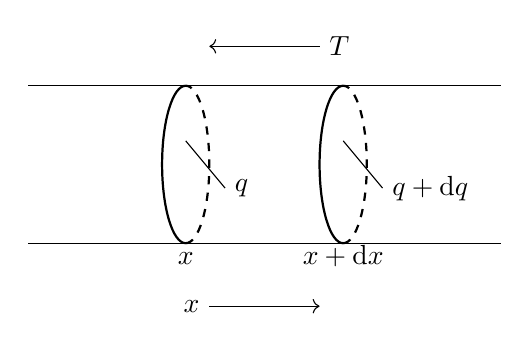
\begin{tikzpicture}
        \draw (0,0)--(6,0);
        \draw (0,2)--(6,2);
        \draw [thick] (2,2) arc (90:270:0.3 and 1);
        \draw [thick, dashed] (2,0) arc (-90:90:0.3 and 1);
        \draw [thick] (4,2) arc (90:270:0.3 and 1);
        \draw [thick, dashed] (4,0) arc (-90:90:0.3 and 1);
        \draw [<-] (2.3,2.5)--(3.7,2.5) node[right]{$ T $};
        \draw [->] (2.3,-0.8) node[left]{$ x $}--(3.7,-0.8);
        \node [below] at(2,0) {$ x $};
        \node [below] at(4,0.1) {$ x+\mathrm{d} x $};
        \draw (2,1.3)--(2.5,0.7) node[right]{$ q $};
        \draw (4,1.3)--(4.5,0.7) node[right]{$ q+\mathrm{d} q $};
    \end{tikzpicture}
    \caption{棒元示意图}
    \label{difx}
\end{figure}

将上式两边对坐标取微分有
\begin{equation}
\frac{\mathrm{d}^2 q}{\mathrm{d} x\mathrm{d} t}=-kA\frac{\mathrm{d}^2 T}{\mathrm{d} x^2}\,\Longrightarrow\,\mathrm{d}\frac{\mathrm{d} q}{\mathrm{d} t}=-kA\frac{\mathrm{d}^2 T}{\mathrm{d} x^2}
\end{equation}

根据能量守恒定律,任一时刻棒元的热平衡方程为
\begin{equation}
C\rho A\mathrm{d} x\frac{\mathrm{d} T}{\mathrm{d} t}=\mathrm{d}\frac{\mathrm{d} q}{\mathrm{d} t}=-kA\frac{\mathrm{d}^2 T}{\mathrm{d} x^2}\mathrm{d} x
\end{equation}
其中$ C,\,\rho $分别为材料的比热容与密度,由此可得热流方程
\begin{equation}
\frac{\mathrm{d} T}{\mathrm{d} t}=D\frac{\mathrm{d}^2 T}{\mathrm{d} x^2}
\end{equation}
其中$ D=\frac{k}{C\rho} $称为热扩散系数。上式的解表示了各点温度随时间的变化,其具体形式取决于边界条件。若令热端温度随时间简谐变化,即
\begin{equation}
T=T_0+T_m\sin\omega t
\end{equation}
另一端用冷水冷却,保持恒定低温$ T_0 $,则上式的解,即棒中各点的温度为
\begin{equation}
T=T_0-\alpha x+T_m\exp\left(-\sqrt{\frac{\omega}{2D}}x\right)\sin\left(\omega t-\sqrt{\frac{\omega}{2D}}x\right)
\end{equation}
其中$ T_0 $为直流成分,$ \alpha $为线性成分的斜率,从上式可以看出:

{\kaishu (a)热端$ (x=0) $处温度按简谐方式变化时,这种变化将以衰减波的形式在棒内向冷端传播,称为热波;}

{\kaishu (b)热波波速$ v=\sqrt{2D\omega} $;}	
{\kaishu (c)热波波长$ \lambda=2\pi\sqrt{\frac{2D}{\omega}} $.}

因此在热端温度变化的角频率已知的情况下,只要测出波速或波长即可计算出$ D $。再由$ D=\frac{k}{C\rho} $计算出材料的热导率$ k $。本实验根据$ v=\sqrt{2D\omega} $可得
\begin{equation}
v^2=2\frac{k}{C\rho}\omega\,\Longrightarrow\,k=\frac{v^2C\rho}{4\pi f}=\frac{v^2C\rho}{4\pi}T
\end{equation}
其中$ f,\,T $分别为热端温度按简谐变化的频率和周期。实现上述测量的关键在于热量在样品中一维传播、热端温度按简谐变化。

\subsection{实验步骤}
\begin{enumerate}
\item 检查各处连接管路是否有堵塞,然后打开水源,从出水口观察流量,要求水流稳定。两个冷却水管在两个样品中是串联的,水流先铝后铜,故而一般先测铜样品,后测铝样品,以免冷却水变热。
\item 打开电源,主机进入工作状态。
\item 打开操作软件,在控制软件中设置热源周期$ T=180\,\mathrm s $,先选用铜样品进行测量。
\item 按下“操作”栏中“测量”按钮,使仪器开始测量工作,在窗口上画出$ T-t $曲线族。测量约40分钟后,系统进入动态平衡,样品内温度动态稳定。此时按下“暂停”,在“文件”菜单中保存相应数据。
\item 换用铝样品重做步骤4。
\item 将实验数据通过网络发送给自己,先关闭测量仪器,再关闭计算机。

\end{enumerate}

\section{第二部分:温度的测量和温度计的设计}

\subsection{实验目的}
\begin{enumerate}
\item 用电位差计测热电偶的温差电动势;
\item 用平衡电桥测热敏电阻和铜电阻的温度特性曲线;
\item 设计非平衡电桥实现对热敏电阻的实时测量。
\end{enumerate}


\subsection{实验仪器与用具}
\subsubsection{DHT-2热学实验装置温控仪}
本实验采用DHT-2型热学实验仪进行温度计的控温,其内装有热电偶温度计、铜电阻温度计、热敏电阻温度计,通过加热丝升温、风扇降温,可以用来测试不同类型温度计的温度特性曲线、确定温度系数等。

使用过程中依次将“信号输入”、“加热电流”依次与加热炉上接口相连,然后连接电源、打开电源开关。

按设定键(S)选择温度位数,用上下键加减数值,连续未按设定键(S)八秒,自动停止闪烁并返回正常显示设定值。设定加热温度后打开面板上的加热电流开关。本次实验中建议加热电流为$ 0.6\,\mathrm A $。
\subsubsection{UJ36a型携带式直流电位差计}
本实验采用UJ36a型携带式直流电位差计测量热电偶的电压。利用补偿法原理测量直流电压(或电动势)和对各种直流毫伏表及电子电位差计进行刻度矫正。

本次实验的实际调节过程中,接入待测电压后将倍率开关拨到“$ \times 0.2 $”,调零检流计,将电键开关拨到“标准”,调节工作电流调节变阻器,使检流计再次指零,将电键开关拨到未知。调节滑线读数盘使得检流计再次置零,那么未知电压读数为
\begin{equation}
U_x=\text{滑线盘读数}\times\text{倍率}
\end{equation}
\subsubsection{DHQJ-5型教学用多功能电桥}
本实验采用DHQJ-5型教学用多功能电桥进行电阻测定与温度计的实时测量,具有开放式电桥、双臂电桥、单臂电桥、功率电桥和非平衡使用的单臂电桥等功能,本次实验主要再单臂电桥下,用平衡电桥测温度计的电阻,用非平衡电桥对温度计进行实时测量。

在平衡电桥下,检流计中的电流与电压均为0,则待测电阻值为
\begin{equation}
R_x=\frac{R_2}{R_1}R_3
\end{equation}

非平衡电桥是单臂电桥在非平衡状态下的一种工程应用。DHQJ-5在非平衡使用时,其造作步骤基本与单臂电桥相同,但测量目的与方法有很大差异,在本次实验中,选用非平衡电桥电压的变化线性表示热敏电阻温度计测量温度的变化。

\subsection{实验原理}
\subsubsection{用电位差计测热电偶的温差电动势}
热电偶又被称作温差电偶,是由A,B两种不同材料的金属丝的端点彼此紧密接触而成的。当两个接点处于不同温度$ t,\,t_0 $时,在回路中会产生直流电动势,该电动势被称为温差电动势或热电动势。当组成热电偶的材料一定时,温差电动势$ E_x $仅与两接点处的温度有关,且两接点的温度在一定温度范围内有如下近似关系式:
\begin{equation}
E_x\approx\alpha(t-t_0)
\end{equation}
其中$ \alpha $称为温差电系数,对于不同金属组成的热电偶,$ \alpha $不同。%其数值上等于两接点温度差为1\,\textcelsius 时产生的电动势。

为了测量温差电动势,就需要将热电偶接入电位差计,但测量仪器的引入不能影响热电偶的性质,故而实验时需保证一定条件。根据伏打定律,即在A,B两种金属之间接入第三种金属C,且其与A,B两接点处于同一温度,这样的闭合回路的温差电动势与上述只有A,B两种金属组成回路中的温差电动势数值完全相同。所以通常将A,B两根化学成分不同的金属丝一端焊接在一起,构成热电偶的热端,将另两端各与铜引线\footnote{即第三种金属C。}焊接,构成两个同温度的冷端。

铜引线与电位差计相连,从而构成了一个热电偶温度计。通常将冷端置于冰水混合物中,保持$ t_0=0 $\,\textcelsius,将热端置于待测温度处,即可测得相应的温差电动势。%再根据事先校正好的曲线或数据来求出温度$ t $。

%	热电偶温度计有点在于热容量小、灵敏度高、反应迅速、测温范围广,还能将温度转换成电学量,因此其再自动测温、控温等系统中得到广泛应用。

\subsubsection{金属电阻温度计}


金属电阻温度计:一般而言,金属电阻随温度的变化规律为
\begin{equation}
R_x=R_{x0}(1+\alpha t+\beta t^2)
\end{equation}
其中$ R_{x0} $为$ t=0 $\,\textcelsius 时的电阻值。如铜电阻的相关参数为
\begin{equation}
R_{x0}=50\,\Omega\qquad \alpha=4.289\times10^{-3}\mathrm{^\circ C}^{-1}\qquad \beta=2.133\times10^{-7}\mathrm{^\circ C}^{-2}
\end{equation}


通常,在温度不是很高的情况下,可忽略温度二次项$ \beta t^2 $,从而可将金属的电阻值随温度的变化看作线性变化,即
\begin{equation}
R_x=R_{x0}(1+\alpha t)=R_{x0}+\alpha tR_{x0}
\end{equation}
利用控温仪将铜电阻的温度控制在一系列的温度值上,待温度稳定后,用平衡电桥测出铜电阻的阻值,画出温度--阻值曲线,进行线性拟合即可求出温度系数。

\subsubsection{半导体热敏温度计}
半导体热敏电阻NTC通常由一些金属氧化物如$ \mathrm{Fe_3O_4} $、$ \mathrm{MgCr_2O_4} $等半导体制成。在这些半导体内部,自由电子数目随着温度升高迅速增加,导电能力的增强很快,所以NTC具有负的电阻温度系数,随着温度升高,其电阻值迅速下降。通过改良也可以设计出正温度系数的热敏电阻,简称PTC。

热敏电阻的电阻温度特性可以用下述指数函数来描述:
\begin{equation}
R_T=A\,e^{B/T}
\end{equation}
式中$ A $是与材料性质的电阻器几何形状有关的常数,$ B $是与材料半导体性质有关的常数,$ T $为绝对温度。

为了求得准确的$ A,B $,可将上式两边取对数:
\begin{equation}\label{2-3-2-2-1}
    \ln R_T=\ln A+\frac BT
\end{equation}
选定不同的温度$ T $,可得到不同的$ R_T $。

当$ T=T_1 $时,有
\begin{equation}
\ln R_{T_1}=\ln A+\frac{B}{T_1}
\end{equation}
当$ T=T_2 $时,有
\begin{equation}
\ln R_{T_2}=\ln A+\frac{B}{T_2}
\end{equation}
将以上两式相减后可得
\begin{equation}\label{2-3-2-2-2}
    B=\frac{\ln R_{T_1}-\ln R_{T_2}}{\frac{1}{T_1}-\frac{1}{T_2}}
\end{equation}
常用半导体热敏电阻的$ B $值约在$ 1500\sim 5000\,\mathrm K $之间。

将式(\ref{2-3-2-2-2})代入式(\ref{2-3-2-2-1})可得
\begin{equation}\label{2-3-2-2-3}
    A=R_{T_1}\,e^{-B/T_1}
\end{equation}

利用控温仪将热敏电阻温度控制在一系列温度点上,用平衡电桥测出相应的电阻,根据式(\ref{2-3-2-2-1})进行线性拟合,可以求出热敏电阻的温度系数$ A,\,B $;若只测两个温度点,也可以通过式(\ref{2-3-2-2-2}) 和 (\ref{2-3-2-2-3})求出$ A,\,B $.




\subsubsection{设计非平衡电桥实现对热敏电阻的实时测量}

\begin{center}
\noindent\begin{minipage}{0.62\columnwidth}
    \hspace*{2em} 非平衡电桥的电路图如右图所示。
    非平衡电桥的测试步骤与平衡电桥一样,只是选用电压表测两端电压,认为电压表内阻无穷大,忽略流过电压表的电流。平衡时电桥电压为0,而非平衡电桥电压$ U_0 $随$ R_x $实时变化,通过计算选取合适的$ R_1,\,R_2,\,R_2 $以及$ E $,让测试电压$ U_0 $随温度$ t $线性变化,则可以对温度进行实时测量。

    可求得:
    \begin{equation}\label{2-3-3-1}
        U_0=\left(\frac{R_x}{R_2+R_x}-\frac{R_3}{R_1+R_3}\right)E
    \end{equation}
    其中:
    \begin{equation}\label{2-3-3-2}
        R_x=A\,e^{B/T}
    \end{equation}
    $ A,B $的值可分别根据式(\ref{2-3-2-2-2}),(\ref{2-3-2-2-3})求得。

\end{minipage}\hfill\begin{minipage}{0.32\columnwidth}
    \begin{figure}[H]
        \centering
        \resizebox{\columnwidth}{!}{
            \begin{circuitikz}
                \draw (0.8,0.5)
                to[short] (0,0)
                to[short,o-] (-2.5,0)
                to[short] (-2.5,3)
                to[short,-*] (-2,3)
                to[european resistor,-*,l={$ R_1 $},a={$ I_1 $}] (0,4.5)
                to[european resistor,-*,l={$ R_3 $},a={$ I_3 $}] (2,3);
                \draw (-2,3)
                to[european resistor,-*,l={$ R_2 $},a={$ I_2 $}] (0,1.5)
                to[european resistor,-*,l={$ R_x $},a={$ I_4 $}] (2,3);
                \draw (0,4.5)
                to[short] (0,5)
                to[short] (3,5)
                to[voltmeter,l={$ U_0 $}] (5,5)
                to[short] (5,1)
                to[short] (0,1)
                to[short] (0,1.5);
                \draw (0.9,0)
                to[battery,o-,a={$ E $}] (3,0)
                to[short] (3,3)
                to[short] (2,3);
                \node[below] at(0.45,0) {$ K $};
            \end{circuitikz}
        }
        \caption{非平衡电桥电路图}
    \end{figure}
\end{minipage}\end{center}


将式(\ref{2-3-3-2})代入式(\ref{2-3-3-1})即可得到$ U_0 $与$ T $间的函数关系,对$ U_0 $作泰勒展开,略去三阶及以上的高阶项,可以得到
\begin{equation}
U_0=U_{01}+U_0'(T-T_1)+U_0''(T-T_1)^2
\end{equation}
其中$ T_1 $为测试区间的中间值,例如监测$ 30\sim 50 $\,\textcelsius 的温度区间,取$ T_1=40\mathrm{^\circ C} $。令$ U_0''=0 $,可得
\begin{equation}\label{28}
    R_x=A\,e^{B/T}=\frac{B+2T}{B-2T}R_2
\end{equation}
那么得到$ U_0 $关于$ T $的线性表达:
\begin{equation}
U_0=\lambda+m(t-t_1)
\end{equation}
其中
\begin{equation}
\lambda=\left(\frac{B+2T_1}{2B}-\frac{R_3}{R_1+R_3}\right)E=U_{01},\quad m=\left(\frac{4T_1^2-B^2}{4BT_1^2}\right)E=U_0'
\end{equation}
由于是温度差,绝对温度$ T $可换成摄氏温度$ t $。而$ \lambda $表示在温度区间中间值时对应的$ U_0 $值,$ m $表示灵敏度。


根据选定的$ \lambda,\,m $,由两个温度点求得$ A,\,B $,以及式(\ref{28})可计算得到$ R_2,\frac{R_1}{R_3},E $,具体表达式如下:
\begin{equation}
E=\left(\frac{4BT_1^2}{4T_1^2-B^2}\right)m,\quad R_2=\frac{B-2T}{B+2T}R_{xT_1},\quad\frac{R_1}{R_3}=\frac{2BE}{(B+2T_1)E-2B\lambda}-1
\end{equation}
根据计算结果即可设定非平衡电桥的相应参数。

\subsection{实验步骤}
\subsubsection{用电位差计测热电偶的温差电动势}
\begin{enumerate}
\item 在室温下测得热电偶的电动势。
\item 开启温控仪电源,对热端加热,在$ 30\sim 50\mathrm{^\circ C} $区间内每隔$ 5\,\mathrm{^\circ C} $测定一组$ (t,E_x) $\footnote{需等温度稳定后进行读数测量。}。
\item 绘制温度特性曲线,通过线性拟合求得温度系数。
\end{enumerate}

\subsubsection{用平衡电桥测热敏电阻和铜电阻的电阻值}
\begin{enumerate}
\item 在室温下测得热敏电阻、铜电阻的电阻值。
\item 在$ 30\sim 50\,\mathrm{^\circ C} $区间内每隔$ 5\mathrm{^\circ C} $测定一组$ (t,R_x) $。
\item 绘制温度特性曲线,通过线性拟合求温度系数。
\end{enumerate}

\subsubsection{用非平衡电桥制作热敏电阻温度计}
选定$ \lambda = -400\,\mathrm{mV},\; m=-10\,\mathrm{mV/\mathrm{^\circ C}},\; t_1=40\mathrm{^\circ C} $,根据在$ 30\mathrm{^\circ C},\;50\mathrm{^\circ C} $下测得的热敏电阻大小计算$ A,\,B $,进而计算$ E,\,R_2,\,\frac{R_1}{R_3} $.

根据计算结果设定非平衡电桥的参数,将温控仪温度设定为$ 40\mathrm{^\circ C} $,微调$ R_2 $阻值,使得电压表测得电压接近$ -400\,\mathrm{mV} $。

改变温控仪温度,在$ 40\sim 50\mathrm{^\circ C} $区间内,每隔$ 2.5\mathrm{^\circ C} $测得一组$ U_0,\,t $,观察自制温度计测温的精度。

















%\newpage
%\subsection*{附录 A\hspace*{20pt} 原始数据记录表}
%\addcontentsline{toc}{section}{附录 A\hspace*{6pt} 原始数据记录表} 
\thispagestyle{fancy} 

\begin{figure}[H]\centering
    %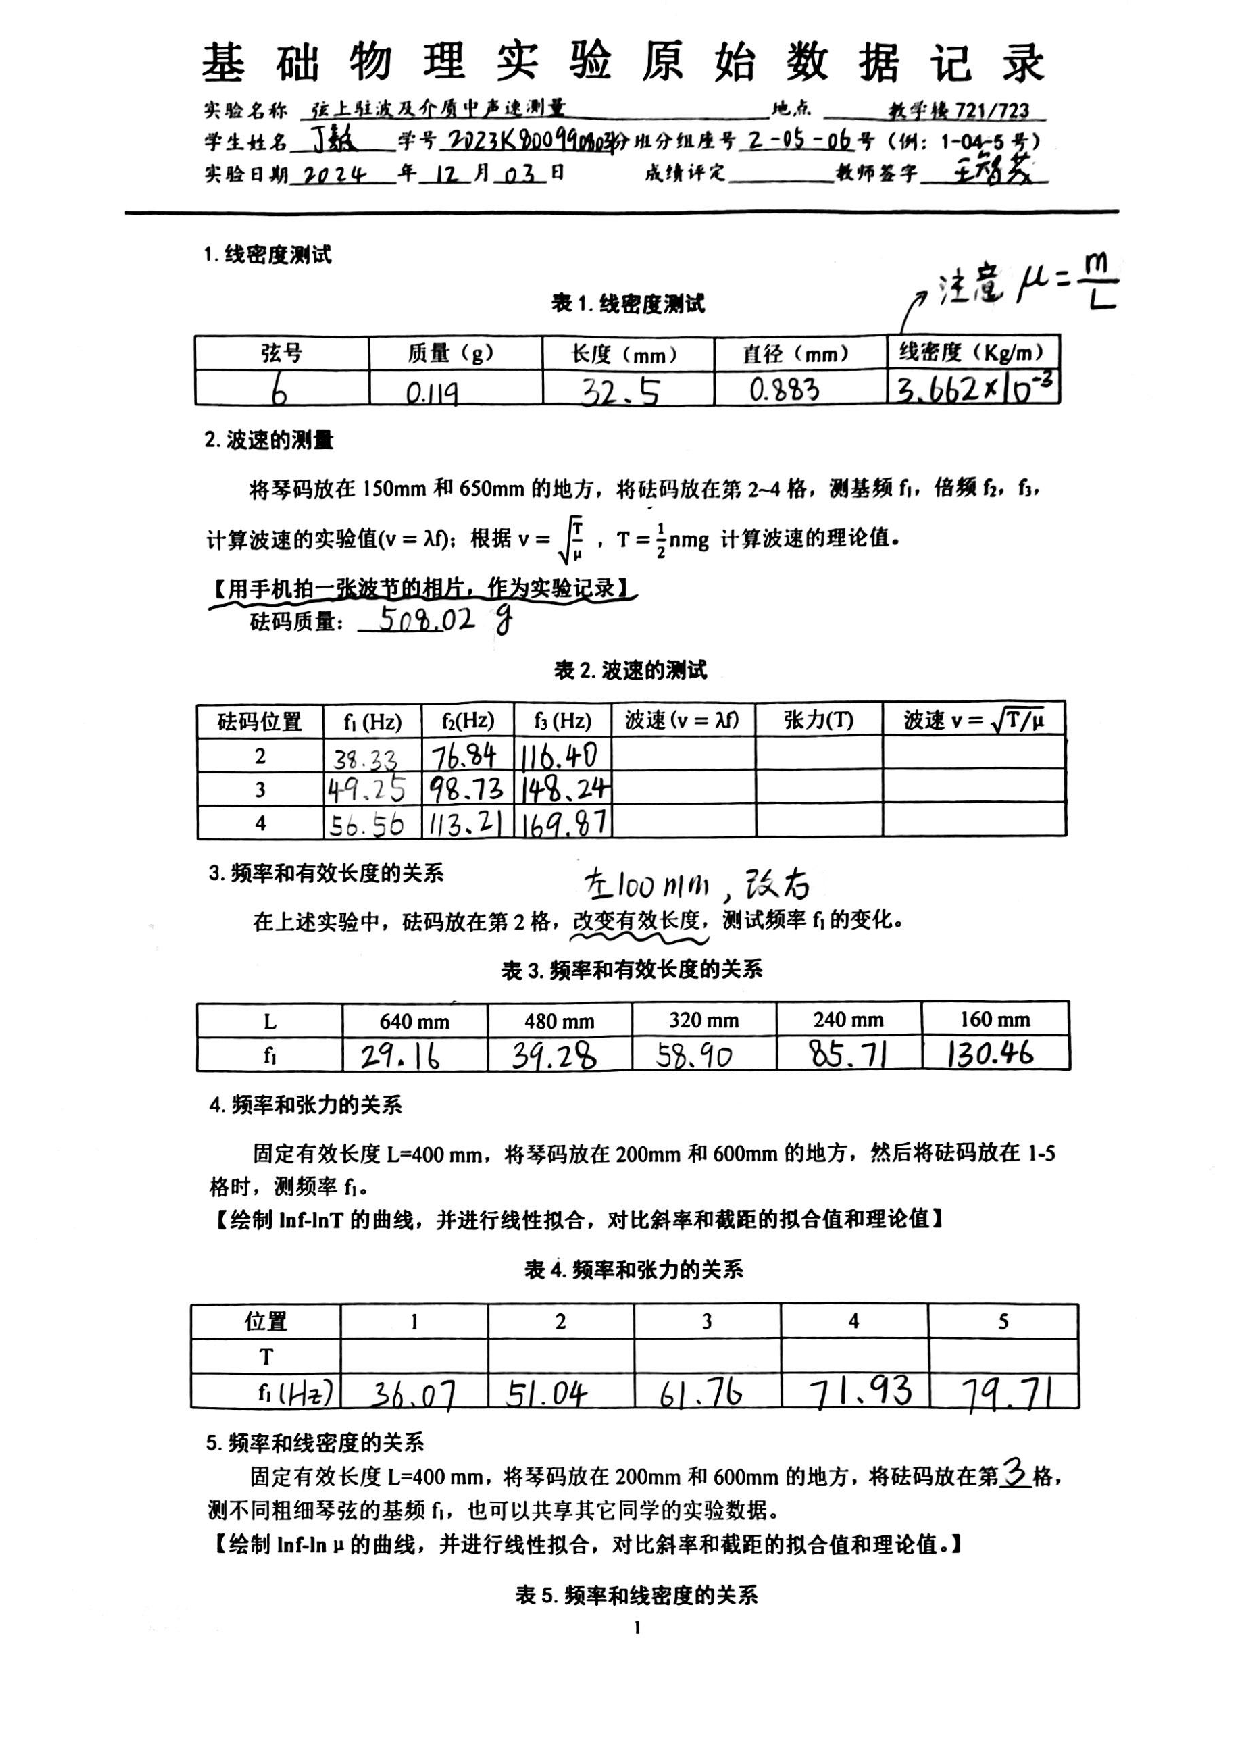
\includepdf[pages=1, width=480pt]{pdf/原始数据-2-05组-丁毅-驻波实验-2024.12.03-王智茂.pdf}
\end{figure}
%includepdf[pages={2}]{pdf/原始数据-2-05组-丁毅-驻波实验-2024.12.03-王智茂.pdf}

%\subsection*{附录 B\hspace*{20pt} Matlab 源码}
%\addcontentsline{toc}{section}{附录 B\hspace*{6pt} Matlab 源码} 
\thispagestyle{fancy} 
%\lstinputlisting{d:/a_RemoteRepo/GH.MatlabCodes/本科课程代码/基础物理实验/Ex_3/Ex_03_mfile.m}

\end{document}

% VScode 常用快捷键:

% F2:                       变量重命名
% Ctrl + Enter:             行中换行
% Alt + up/down:            上下移行
% 鼠标中键 + 移动:           快速多光标
% Shift + Alt + up/down:    上下复制
% Ctrl + left/right:        左右跳单词
% Ctrl + Backspace/Delete:  左右删单词    
% Shift + Delete:           删除此行
% Ctrl + J:                 打开 VScode 下栏(输出栏)
% Ctrl + B:                 打开 VScode 左栏(目录栏)
% Ctrl + `:                 打开 VScode 终端栏
% Ctrl + 0:                 定位文件
% Ctrl + Tab:               切换已打开的文件(切标签)
% Ctrl + Shift + P:         打开全局命令(设置)

% Latex 常用快捷键:

% Ctrl + Alt + J:           由代码定位到PDF


